\documentclass[border=4pt]{standalone}
\usepackage{fontspec}
\setmainfont{TeX Gyre Heros}\setsansfont{TeX Gyre Heros}\setmonofont{TeX Gyre Cursor}
\usepackage{tikz}
\usetikzlibrary{arrows.meta}
\definecolor{palRose}{HTML}{CC6677}
\tikzset{
 call/.style   ={-{Stealth[length=1.6mm,width=1.2mm]}, black!60, line width=0.6pt},
 ret/.style    ={call, dashed},
 async/.style  ={-{Straight Barb[length=2mm,width=2mm]}, black!60, line width=0.6pt},
 syncm/.style  ={-{Triangle[length=2mm,width=1.6mm]}, black!60, line width=0.6pt},
 dep/.style    ={async, dashed},
 gen/.style    ={-{Triangle[length=3mm,width=3mm,fill=white,line width=0.6pt]}, black!60, line width=0.6pt},
 real/.style   ={gen, dashed},
 aggr/.style   ={{Diamond[length=3mm,width=2mm,fill=white,line width=0.6pt]}-, black!60, line width=0.6pt},
 comp/.style   ={{Diamond[length=3mm,width=2mm]}-, black!60, line width=0.6pt},
 found/.style  ={{Circle[length=1.6mm]}-{Stealth[length=1.6mm,width=1.2mm]}, black!60, line width=0.6pt},
 lost/.style   ={-{Stealth[length=1.6mm,width=1.2mm]Circle[length=1.6mm]}, black!60, line width=0.6pt},
 verify/.style ={-{Stealth[length=1.6mm,width=1.2mm]Bar[width=2.5mm]}, black!60, line width=0.6pt},
 blocked/.style={-{Bar[width=2.5mm]}, dashed, draw=palRose, line width=0.8pt},
 busline/.style={double, double distance=1.2pt, draw=black!45},
 bidir/.style  ={{Stealth[length=1.6mm,width=1.2mm]}-{Stealth[length=1.6mm,width=1.2mm]}, black!60, line width=0.6pt},
 maps/.style   ={{Hooks[length=0.8mm,width=1.6mm]}-{Stealth[length=1.6mm,width=1.2mm]}, black!60, line width=0.6pt},
 trust/.style  ={dotted, -{Straight Barb[length=2mm,width=2mm]}, black!60, line width=0.8pt},
 emph/.style   ={call, line width=1.1pt},
 boundary/.style={draw=black!80, line width=1.4pt},
}
\begin{document}
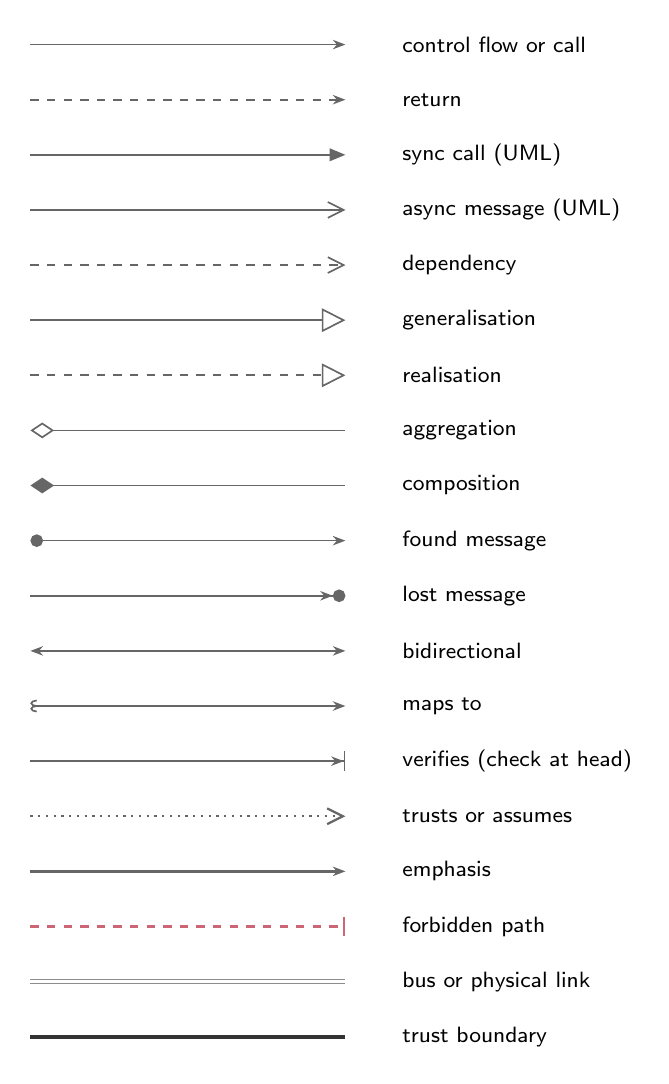
\begin{tikzpicture}[x=1mm,y=1mm,font=\sffamily\footnotesize]
\foreach \s/\l [count=\i] in {call/control flow or call,ret/return,syncm/sync call (UML),async/async message (UML),dep/dependency,gen/generalisation,real/realisation,aggr/aggregation,comp/composition,found/found message,lost/lost message,bidir/bidirectional,maps/maps to,verify/verifies (check at head),trust/trusts or assumes,emph/emphasis,blocked/forbidden path,busline/bus or physical link,boundary/trust boundary}{
 \draw[\s] (0,-7*\i) -- (40,-7*\i);
 \node[anchor=west] at (46,-7*\i) {\l};
}
\end{tikzpicture}
\end{document}
